\documentclass[10pt, aspectratio=169]{beamer}

%======================================================
% Theme (matches Lectures 9/10/11)
%======================================================
\usetheme[progressbar=frametitle, sectionpage=progressbar, subsectionpage=progressbar, numbering=fraction, block=fill]{metropolis}

\definecolor{mLightBrown}{HTML}{4D4D4D}
\definecolor{mMediumBrown}{HTML}{2C2C2A}
\definecolor{mDarkBrown}{HTML}{1A1A19}
\definecolor{mDarkTeal}{HTML}{0F6E56}
\definecolor{mDarkRed}{HTML}{B03A2E}
\setbeamercolor{normal text}{fg=mDarkBrown}
\setbeamercolor{alerted text}{fg=mDarkTeal}
\setbeamercolor{frametitle}{bg=mDarkBrown}
\setbeamercolor{progress bar}{fg=mDarkTeal, bg=mDarkTeal!20}

\definecolor{mPaleBg}{HTML}{F4F3EE}
\setbeamercolor{block title}{bg=mDarkBrown!10, fg=mDarkBrown}
\setbeamercolor{block body}{bg=mPaleBg, fg=mDarkBrown}
\newcommand{\hl}[1]{\textcolor{mDarkTeal}{#1}}

%======================================================
\usepackage{amsmath, amssymb, amsthm, mathtools}
\usepackage{cancel}
\usepackage{bm}
\usepackage{booktabs}
\usepackage{array}
\usepackage{xcolor}
\usepackage{colortbl}
\usepackage{multirow}
\usepackage{tikz}
\usetikzlibrary{positioning,arrows.meta,calc,fit,shapes.geometric,decorations.pathmorphing}

%======================================================
\newcommand{\paper}[1]{\textcolor{mLightBrown}{\small\textit{(#1)}}}

% --- the recurring four-question strip ---------------
\newcommand{\qcur}{0}
\newcommand{\qnode}[4]{%
\ifnum#4=\qcur
 \node[draw=mDarkTeal, fill=mDarkTeal!12, thick, rounded corners=1pt, minimum width=3.0cm, minimum height=0.52cm, font=\tiny\bfseries, text=mDarkBrown] (#2) at (#1,0) {#3};%
\else
 \node[draw=mLightBrown!45, rounded corners=1pt, minimum width=3.0cm, minimum height=0.52cm, font=\tiny, text=mLightBrown] (#2) at (#1,0) {#3};%
\fi}
\newcommand{\qstrip}[1]{\renewcommand{\qcur}{#1}%
\begin{center}
\begin{tikzpicture}
\qnode{0}{q1}{Q1 Evaluate?}{1}
\qnode{3.7}{q2}{Q2 Improve?}{2}
\qnode{7.4}{q3}{Q3 Explore?}{3}
\qnode{11.1}{q4}{Q4 Scale?}{4}
\draw[-{Stealth}, mLightBrown!60] (q1.east) -- (q2.west);
\draw[-{Stealth}, mLightBrown!60] (q2.east) -- (q3.west);
\draw[-{Stealth}, mLightBrown!60] (q3.east) -- (q4.west);
\end{tikzpicture}\end{center}}

%======================================================
\title{Value-Based Reinforcement Learning}
\subtitle{Learning to act when the model is gone}
\author{Jinkyoo Park}
\institute{KAIST}
\date{\textit{Lecture 8 --- From the Bellman equation you can solve to the one you can only sample}}

%======================================================
\begin{document}
%======================================================

\maketitle

%==========================================================
\section{The handoff --- what Lecture 7 left us}
%==========================================================

\begin{frame}{Where we are --- the OR lineage, made data-driven}
\vspace{2pt}
\begin{center}\footnotesize
\renewcommand{\arraystretch}{1.35}
\begin{tabular}{r|c|c}
 & \textbf{OR / Dynamic Programming} & \textbf{Control Theory} \\
\hline
\textbf{Model-based (origin)}  & MDP \& DP \scriptsize(Lec.\ 7) & Optimal Control \scriptsize(Lec.\ 9)\\
\hline
\textbf{Data-driven (extension)} & \cellcolor{mDarkTeal!20}\textbf{Value-Based RL} \scriptsize(\alert{Lec.\ 8}) & Policy-Based RL \scriptsize(Lec.\ 10)\\
\end{tabular}
\end{center}
\smallskip

This lecture is the \alert{bottom-left cell}: the data-driven extension of the operations-research lineage. Lecture 7 (MDP \& DP) was its model-based origin; we now do to it the one move that defines this half of the course --- \alert{delete the model and learn from samples}. (Lecture 10 will do the identical move to the control lineage.)
\smallskip

We stay in the same cell of the big map --- \textbf{single agent, multiple stages} --- and move along one axis only: from a world we are \alert{handed} ($P$, $R$ known) to a world we can only \alert{sample}.
\smallskip

\pause
What Lecture 7 gave us, stated as one object --- the \alert{Bellman optimality equation}:
\[
Q^*(s,a) \;=\; \sum_{s'} \hl{P(s'\mid s,a)}\Big[\,\hl{R(s,a,s')} + \gamma \max_{a'} Q^*(s',a')\,\Big].
\]
\smallskip

\pause
And two ways to solve it --- value iteration, policy iteration. Both are exact. Both are \alert{useless without the two highlighted terms}.
\end{frame}

\begin{frame}{What we keep, and what we lose}
The fixed point of this lecture, in one line:
\begin{center}\large
\alert{The Bellman equation survives. The model does not.}
\end{center}
\medskip

\pause
Everything else follows from removing $P$ and $R$. Three things break the moment they vanish:
\begin{itemize}\setlength\itemsep{3pt}
\item \textbf{The expectation.} $\sum_{s'} P(s'\mid s,a)\,[\cdots]$ cannot be computed --- we never see $P$, only one sampled $s'$ at a time.
\item \textbf{The improvement step.} Acting greedily on $V$ needs $P$ to look one step ahead. Without it, $V$ alone cannot tell us \emph{what to do}.
\item \textbf{The table.} Even with samples, a $Q$-value per state--action pair does not fit in memory --- nor generalize --- once states are images.
\end{itemize}
\medskip

\pause
Each break is one question of today. We never replace the Bellman equation; we replace the \emph{model inside it} --- first by samples, then by a function.
\end{frame}

\begin{frame}{The translation table --- our coordinate system for today}
Every object of Lecture 7 has a \emph{sampled} counterpart. Keep this in sight.
\medskip
\begin{center}\scriptsize\renewcommand{\arraystretch}{1.55}
\begin{tabular}{l|l|l}
\textbf{Lecture 7 (model-based)} & \textbf{Lecture 8 (sampled)} & \textbf{What replaces the model} \\
\hline
expectation $\sum_{s'} P(s'\mid s,a)[\cdots]$ & one transition $(s,a,r,s')$ & a sample average / a bootstrap \\
policy evaluation (solve with $P,R$) & MC or TD prediction & returns, or a one-step estimate \\
greedy on $V$: $\arg\max_a \sum_{s'}P[\cdots]$ & greedy on $Q$: $\arg\max_a Q(s,a)$ & store $Q$, not $V$ \\
value iteration & Q-learning & $\max$ inside a sampled backup \\
full backup (all successors) & sample backup (one successor) & the law of large numbers \\
tabular, exact & function approximation (DQN) & a network $Q(s,a;w)$ \\
\end{tabular}
\end{center}
\medskip

\pause
Read column~3. Nothing here is a new \emph{principle} --- it is the same Bellman backup, with the one piece we don't own quietly swapped out. The art is in \alert{what we swap it for} without the whole thing collapsing.
\end{frame}

\begin{frame}{One honest detour --- why not just learn the model?}
The most literal idea: estimate $P,R$ from data, then run Lecture 7.
\[
\hat P(s'\mid s,a) = \frac{\#(s,a,s')}{\#(s,a)}, \qquad
\hat R(s,a,s') = \text{average } r \text{ over } (s,a,\cdot,s').
\]
Plug in, solve the MDP. This is \alert{model-based RL}, and it is perfectly valid.
\medskip

\pause
But notice the waste: to choose actions we only ever need $Q^*$, yet here we first estimate a \emph{whole transition kernel} --- vastly more parameters than the thing we actually use. Why estimate $P$ and $R$ at all,
\begin{center}\large
\alert{when we could estimate $Q^*$ directly?}
\end{center}
\medskip

\pause
That question --- \emph{skip the model, estimate the value} --- is the entire model-free programme. The rest of today walks it. \hfill {\footnotesize\textcolor{mLightBrown}{(The model returns, deliberately, in Lecture 10.)}}
\end{frame}

\begin{frame}{The roadmap --- four questions}
One question per Act. This strip returns at every transition --- watch the highlight move.
\qstrip{0}
\medskip
\begin{itemize}\setlength\itemsep{3pt}
\item \textbf{Q1 --- How do we evaluate a policy with no model?} Sample the whole return, or \alert{bootstrap} from one step. \paper{MC vs.\ TD; Sutton, 1988}
\item \textbf{Q2 --- How do we improve with no model?} Greedy-on-$V$ needs $P$; so learn \alert{$Q$}, and pay for exploration with $\varepsilon$-greedy.
\item \textbf{Q3 --- Whose value are we learning?} On-policy (\alert{SARSA}) vs.\ off-policy (\alert{Q-learning}) --- the cliff decides. \paper{Watkins, 1989}
\item \textbf{Q4 --- Can it scale past a table?} Function approximation, the deadly triad, and the two tricks of \alert{DQN}. \paper{Mnih et al., 2013/2015}
\end{itemize}
\end{frame}

%==========================================================
\section{Act 1 --- evaluation without a model}
%==========================================================

\begin{frame}{The arena --- from MDP to experience}
We no longer query a model. We \emph{act}, and a stream comes back:
\[
s_1, a_1, r_2, s_2, a_2, r_3, s_3, \dots, s_T \qquad (\text{one episode}).
\]
\begin{itemize}\setlength\itemsep{2pt}
\item the agent chooses $a_t = \pi(s_t)$ --- \emph{decision},
\item the environment returns $r_{t+1}, s_{t+1}$ --- \emph{the only window onto $P,R$},
\item from this stream we must recover $Q^*$ and act on it --- \emph{learning}.
\end{itemize}
\medskip

\pause
Start with the humblest sub-task: \alert{prediction}. Fix a policy $\pi$; estimate its value $V^\pi$. No control yet --- just: how good is this behavior? Everything harder is built on getting this right.
\end{frame}

\begin{frame}{The quantity, and the two ways to estimate it}
The definition has not changed since Lecture 7 --- only our access to it:
\[
V^\pi(s) = \mathbb{E}_\pi\!\big[\,G_t \mid s_t = s\,\big]
 = \underbrace{\mathbb{E}_\pi\!\big[\textstyle\sum_{k\ge0}\gamma^k r_{t+k+1}\mid s_t=s\big]}_{\text{\hl{the full return}}}
 = \underbrace{\mathbb{E}_\pi\!\big[r_{t+1}+\gamma V^\pi(s_{t+1})\mid s_t=s\big]}_{\text{\hl{one step, then bootstrap}}}.
\]
\medskip

The same value, written two ways. Each writing is a recipe for estimating it from samples:
\begin{itemize}\setlength\itemsep{2pt}
\item \textbf{Monte Carlo} reads the \emph{left} form: wait for the episode to end, average the realized return $G_t$.
\item \textbf{Temporal Difference} reads the \emph{right} form: take one step, then \alert{trust your own current estimate} of the rest.
\end{itemize}
\medskip

\pause
The split between them --- \emph{sample the whole thing} vs.\ \emph{sample one step and bootstrap} --- is the deepest fork in all of value-based RL. Watch it return in every algorithm.
\end{frame}

\begin{frame}{Monte Carlo prediction --- average what actually happened}
Visit $s_t$, watch the episode finish, collect the realized return $G_t = r_{t+1}+\gamma r_{t+2}+\cdots+\gamma^{T-t-1}r_T$. Then nudge:
\[
V(s_t) \;\leftarrow\; V(s_t) + \alpha\big[\,\underbrace{G_t}_{\text{target}} - V(s_t)\,\big].
\]
\medskip
\begin{itemize}\setlength\itemsep{2pt}
\item \textbf{Unbiased.} $\mathbb{E}[G_t] = V^\pi(s_t)$ exactly --- the target is the real thing, not a guess.
\item \textbf{No model, no bootstrap.} Each state's estimate stands alone; we never lean on neighbors.
\item \textbf{The price:} must wait for the terminal state (no online updates), and the return of a long episode is a \alert{high-variance} single draw --- one unlucky tail corrupts the estimate.
\end{itemize}
\medskip

\pause
{\footnotesize\textcolor{mLightBrown}{MC also ``wastes'' the structure of the MDP: it learns each state separately and never reuses the fact that $s$ leads to $s'$. That wasted structure is exactly what TD reclaims.}}
\end{frame}

\begin{frame}{Temporal Difference --- learn a guess from a guess}
Don't wait. After a \emph{single} transition $(s_t, r_{t+1}, s_{t+1})$, update:
\[
V(s_t) \;\leftarrow\; V(s_t) + \alpha\big[\,\underbrace{r_{t+1} + \gamma V(s_{t+1})}_{\text{\alert{TD target}}} - V(s_t)\,\big].
\]
\medskip
The target contains $V(s_{t+1})$ --- \alert{our own current estimate}. We update a guess toward a slightly-better guess. This is \textbf{bootstrapping}.
\medskip

\pause
\begin{itemize}\setlength\itemsep{2pt}
\item \textbf{Online, incremental, model-free.} One step is enough --- ideal for long or non-terminating tasks.
\item \textbf{Low variance, some bias.} The target depends on one reward plus a learned value, not a whole noisy trajectory --- but it inherits whatever error $V(s_{t+1})$ currently carries.
\item In practice TD usually converges \emph{faster} than constant-$\alpha$ MC on stochastic tasks.
\end{itemize}
\end{frame}

\begin{frame}{The triangle --- MC, DP, and TD}
Three ways to back up a value; TD is the one that takes from both parents.
\medskip
\begin{center}\scriptsize\renewcommand{\arraystretch}{1.3}
\begin{tabular}{l|c|c}
 & \textbf{Samples (no model)} & \textbf{Bootstraps (uses own estimate)} \\
\hline
\textbf{Dynamic Programming} (Lec.\ 7) & \textcolor{mDarkRed}{no} --- needs full $P$ & yes \\
\textbf{Monte Carlo} & yes & \textcolor{mDarkRed}{no} --- waits for true return \\
\rowcolor{mDarkTeal!12}\textbf{Temporal Difference} & \textbf{yes} & \textbf{yes} \\
\end{tabular}
\end{center}
\medskip

\pause
\begin{center}\large
\alert{TD = the model-free-ness of MC $+$ the bootstrapping of DP.}
\end{center}
\medskip
That single inheritance is why TD, not MC, becomes the engine of control. We now turn the prediction crank into a \emph{decision-making} one.
\end{frame}

%==========================================================
\section{Act 2 --- improvement without a model}
%==========================================================

\begin{frame}{Why $V$ is not enough --- the hidden $P$}
\qstrip{2}
\medskip
Lecture 7's improvement step, written out:
\[
\pi'(s) = \arg\max_a \sum_{s'} \hl{P(s'\mid s,a)}\big[R(s,a,s') + \gamma V(s')\big].
\]
To turn a \emph{value} into an \emph{action}, you must look one step ahead --- and looking ahead needs the model.
\medskip

\pause
The fix is almost embarrassingly simple. Store the action-value $Q$ instead of $V$:
\[
\pi'(s) = \arg\max_a \; \hl{Q(s,a)}.
\]
No sum, no $P$. \alert{$Q$ already has the look-ahead baked in.} This is \emph{the} reason value-based RL learns $Q$, not $V$: $Q$ is the model-free currency of decisions.
\end{frame}

\begin{frame}{Generalized Policy Iteration, now from samples}
The Lecture 7 dance is unchanged --- evaluate, improve, repeat --- but each half is now sampled.
\medskip
\begin{center}
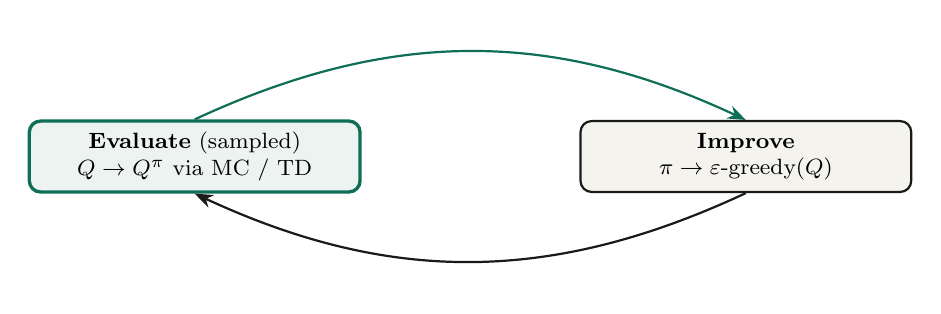
\begin{tikzpicture}[font=\footnotesize, node distance=10pt]
\node[draw=mDarkTeal, very thick, fill=mDarkTeal!8, rounded corners, minimum width=4.2cm, minimum height=0.9cm, align=center] (eval) at (0,0) {\textbf{Evaluate} (sampled)\\ $Q \to Q^\pi$ via MC / TD};
\node[draw=mDarkBrown, thick, fill=mPaleBg, rounded corners, minimum width=4.2cm, minimum height=0.9cm, align=center] (impr) at (7,0) {\textbf{Improve}\\ $\pi \to \varepsilon\text{-greedy}(Q)$};
\draw[-{Stealth}, mDarkTeal, thick] (eval.north) to[bend left=25] (impr.north);
\draw[-{Stealth}, mDarkBrown, thick] (impr.south) to[bend left=25] (eval.south);
\end{tikzpicture}
\end{center}
\medskip

\pause
One subtlety the model-based version never faced: to estimate $Q^\pi(s,a)$ from data, \emph{every} $(s,a)$ must actually be tried. A purely greedy policy never tries the actions it currently dislikes --- and so never learns they were good.
\medskip
\begin{center}\large
\alert{Improvement now requires exploration. That is the new tax.}
\end{center}
\end{frame}

\begin{frame}{The tax, paid: $\varepsilon$-greedy --- and the bandit underneath}
The simplest way to keep trying everything:
\[
a_t = \begin{cases} \arg\max_a Q(s_t,a) & \text{with prob. } 1-\varepsilon \quad(\text{\hl{exploit}})\\[2pt] \text{a random action} & \text{with prob. } \varepsilon \quad(\text{\hl{explore}}).\end{cases}
\]
\medskip

\pause
This is the \alert{exploration--exploitation trade-off} of the $n$-armed bandit, now living inside every state. The bandit was RL with the dynamics deleted; here the dynamics are back, but the same dilemma --- \emph{spend on what you know, or pay to learn more} --- governs every step.
\medskip

\pause
\begin{itemize}\setlength\itemsep{1pt}
\item Decay $\varepsilon \to 0$ (e.g.\ $\varepsilon = 1/t$) and, with every $(s,a)$ visited infinitely often, the greedy policy in the limit is optimal.
\item Hold $\varepsilon$ fixed and you keep a permanently-cautious, permanently-curious agent --- sometimes exactly what a real system needs.
\end{itemize}
\end{frame}

%==========================================================
\section{Act 3 --- whose value? on-policy vs off-policy}
%==========================================================

\begin{frame}{Two control rules, one tiny difference}
\qstrip{3}
\medskip
Put TD evaluation of $Q$ together with $\varepsilon$-greedy improvement. Two natural updates appear, differing in \emph{one term}:
\medskip
\begin{center}\footnotesize\renewcommand{\arraystretch}{1.6}
\begin{tabular}{l|l}
\textbf{SARSA} (on-policy) & \textbf{Q-learning} (off-policy) \\
\hline
$Q(s,a)\!\leftarrow\! Q(s,a)+\alpha\big[r+\gamma\, \hl{Q(s',a')} - Q(s,a)\big]$ & $Q(s,a)\!\leftarrow\! Q(s,a)+\alpha\big[r+\gamma\, \hl{\max_{a'} Q(s',a')} - Q(s,a)\big]$ \\
$a'$ is the action \emph{actually taken} next & $\max$ over \emph{all} next actions, taken or not \\
\end{tabular}
\end{center}
\medskip

\pause
$\textbf{S},\textbf{A},\textbf{R},\textbf{S}',\textbf{A}'$ --- SARSA literally uses the next action it sampled. Q-learning replaces that sampled $a'$ with the \alert{best possible} $a'$. That single $\max$ is the entire on/off-policy distinction.
\end{frame}

\begin{frame}{The 2$\times$2 that organizes everything}
Cross the two forks of the whole lecture --- \emph{bootstrap?} and \emph{whose policy?}
\medskip
\begin{center}\footnotesize\renewcommand{\arraystretch}{1.5}
\begin{tabular}{r|c|c}
 & \textbf{Non-bootstrap (MC)} & \textbf{Bootstrap (TD)} \\
\hline
\textbf{On-policy}  & MC control & \cellcolor{mDarkTeal!12}\textbf{SARSA} \\
\hline
\textbf{Off-policy} & off-policy MC & \cellcolor{mDarkTeal!12}\textbf{Q-learning} \\
\end{tabular}
\end{center}
\medskip

\pause
\textbf{On-policy:} the policy that \emph{generates} the data is the policy we \emph{evaluate}. SARSA learns the value of the very (exploring, $\varepsilon$-greedy) behavior it is running.
\medskip

\textbf{Off-policy:} the behavior policy and the target policy differ. Q-learning \emph{behaves} $\varepsilon$-greedily but \emph{learns} the value of the pure-greedy optimal policy --- it studies one policy while living as another.
\end{frame}

\begin{frame}{Why Q-learning is ``off-policy,'' precisely}
Look at what each update assumes about the next step.
\medskip
\begin{itemize}\setlength\itemsep{3pt}
\item SARSA's target uses $Q(s',a')$ where $a' \sim \pi_{\text{behavior}}$ --- the \alert{real} next action, exploration and all. It is honest about the policy it runs.
\item Q-learning's target uses $\max_{a'} Q(s',a')$ --- it \emph{pretends} the next action will be greedy, regardless of the $a'$ actually taken. The behavioral $a'$ is collected, then \alert{ignored}.
\end{itemize}
\medskip

\pause
\begin{block}{The clean extreme \hfill {\scriptsize\normalfont act with $\varepsilon=1$, i.e.\ fully random}}
\centering
SARSA learns the value of \emph{acting randomly}. \quad Q-learning learns the value of the \emph{optimal} policy --- \emph{while acting randomly}.
\end{block}
\medskip
Because the learned target is independent of the behavior, $Q$ converges to $Q^*$ no matter how (sufficiently exploratory) the data was gathered.
\end{frame}

\begin{frame}{The cliff --- where the difference becomes visible}
A gridworld: a safe-but-long path, and a fast path hugging a cliff. One wrong step off the cliff is catastrophic.
\medskip
\begin{center}
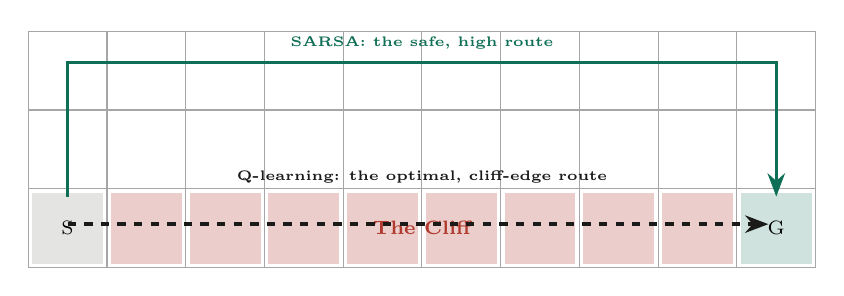
\begin{tikzpicture}[font=\scriptsize]
\draw[mLightBrown!50] (0,0) grid (10,3);
\node[fill=mDarkBrown!12, minimum width=0.9cm, minimum height=0.9cm] at (0.5,0.5) {S};
\node[fill=mDarkTeal!20, minimum width=0.9cm, minimum height=0.9cm] at (9.5,0.5) {G};
\foreach \x in {1.5,2.5,3.5,4.5,5.5,6.5,7.5,8.5} \node[fill=mDarkRed!25, minimum width=0.9cm, minimum height=0.9cm] at (\x,0.5) {};
\node[mDarkRed, font=\scriptsize\bfseries] at (5,0.5) {The Cliff};
\draw[-{Stealth}, mDarkTeal, very thick] (0.5,0.9) -- (0.5,2.6) -- (9.5,2.6) -- (9.5,0.9);
\node[mDarkTeal, font=\tiny\bfseries] at (5,2.85) {SARSA: the safe, high route};
\draw[-{Stealth}, mDarkBrown, very thick, dashed] (0.5,0.55) -- (9.4,0.55);
\node[mDarkBrown, font=\tiny\bfseries] at (5,1.15) {Q-learning: the optimal, cliff-edge route};
\end{tikzpicture}
\end{center}
\medskip

\pause
\begin{itemize}\setlength\itemsep{1pt}
\item \textbf{Q-learning} learns the \emph{optimal} path --- along the edge. But it \emph{acts} $\varepsilon$-greedily; the occasional random step plunges it off the cliff. Higher reward in theory, worse on-line.
\item \textbf{SARSA} accounts for its own exploration --- it knows a random step near the edge is fatal --- so it learns a \alert{cautious} route, away from the cliff. Lower theoretical optimum, safer in practice.
\end{itemize}
\medskip
\pause
{\footnotesize\textcolor{mLightBrown}{Neither is ``better.'' The cliff teaches the design choice: \emph{do you want the optimal policy, or the best policy given that you must keep exploring?}}}
\end{frame}

%==========================================================
\section{Act 4 --- scaling past the table}
%==========================================================

\begin{frame}{The wall --- a table cannot hold the world}
\qstrip{4}
\medskip
Everything so far stores one number per $(s,a)$. Then comes Atari:
\[
\text{state} = \text{four } 84\times84 \text{ grayscale frames} \;\Rightarrow\; |\mathcal{S}| \approx 256^{\,84\times84\times4},
\]
more configurations than atoms in the universe. A $Q$-table is impossible three times over:
\begin{itemize}\setlength\itemsep{1pt}
\item too many states to \emph{visit},
\item too many to \emph{store},
\item and --- fatally --- no \alert{generalization}: a table says nothing about a state it has never seen.
\end{itemize}
\medskip

\pause
The machine-learning answer: stop storing, start \emph{approximating}. Replace the table with a parameterized function.
\[
Q(s,a) \;\approx\; \hat Q(s,a;w), \qquad \text{e.g.\ } \hat Q(s,a;w)=w^\top \phi(s,a) \text{ or a neural net.}
\]
Now ``learning'' means fitting $w$ --- and similar states share answers.
\end{frame}

\begin{frame}{Q-learning as regression --- the semi-gradient step}
Treat the Bellman target as a label and minimize squared error on each transition:
\[
\mathcal{L}(w) = \tfrac12\Big(\underbrace{r + \gamma \max_{a'} \hat Q(s',a';w)}_{\text{target}} - \hat Q(s,a;w)\Big)^2
\;\Rightarrow\;
w \leftarrow w + \alpha\,\delta\,\nabla_w \hat Q(s,a;w),
\]
with TD error $\delta = r + \gamma \max_{a'} \hat Q(s',a';w) - \hat Q(s,a;w)$.
\medskip

\pause
It is called a \alert{semi-gradient} method for an honest reason: we differentiate the prediction $\hat Q(s,a;w)$ but \emph{treat the target as fixed}, even though it too depends on $w$. We are chasing a target that moves when we move.
\medskip

\pause
In the tabular world that chase still converged. With function approximation, it can \alert{diverge}. Tabular Q-learning's guarantees do not survive the jump --- and we must understand why before trusting a network.
\end{frame}

\begin{frame}{The deadly triad --- why naive Deep Q-learning blows up}
Three ingredients are each harmless alone. Together they can make value estimates diverge.
\medskip
\begin{center}
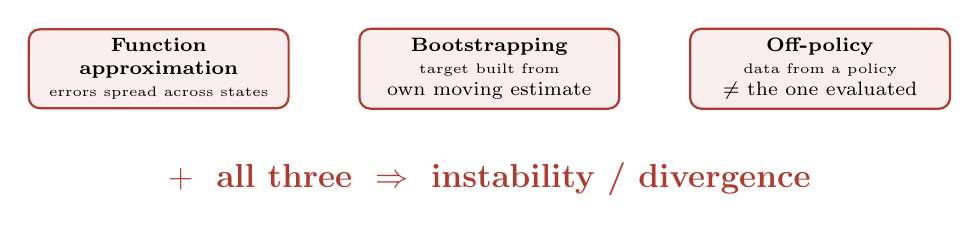
\begin{tikzpicture}[font=\scriptsize, node distance=6pt]
\node[draw=mDarkRed, thick, fill=mDarkRed!8, rounded corners, minimum width=3.3cm, minimum height=1.0cm, align=center] (a) at (0,0) {\textbf{Function}\\\textbf{approximation}\\\tiny errors spread across states};
\node[draw=mDarkRed, thick, fill=mDarkRed!8, rounded corners, minimum width=3.3cm, minimum height=1.0cm, align=center] (b) at (4.2,0) {\textbf{Bootstrapping}\\\tiny target built from\\ own moving estimate};
\node[draw=mDarkRed, thick, fill=mDarkRed!8, rounded corners, minimum width=3.3cm, minimum height=1.0cm, align=center] (c) at (8.4,0) {\textbf{Off-policy}\\\tiny data from a policy\\ $\neq$ the one evaluated};
\node[mDarkRed, font=\large\bfseries] at (4.2,-1.4) {$+$ \;all three\; $\Rightarrow$\; instability / divergence};
\end{tikzpicture}
\end{center}
\medskip

\pause
Q-learning with a neural net has \emph{all three}. The data are also strongly \alert{correlated} (consecutive frames) and the target \alert{shifts} on every update. Plain SGD on $\mathcal{L}(w)$ fights itself.
\medskip
\begin{center}\large
The breakthrough was not a new objective --- it was \alert{two engineering tricks} that tame the triad.
\end{center}
\end{frame}

\begin{frame}{DQN --- the two tricks \hfill {\scriptsize\normalfont \paper{Mnih et al., 2013; Nature 2015}}}
Keep Q-learning's update. Add two stabilizers.
\medskip
\begin{itemize}\setlength\itemsep{4pt}
\item \textbf{Experience replay.} Store transitions $(s,a,r,s')$ in a buffer $D$; train on \emph{random minibatches} from it. This \alert{breaks correlation} between consecutive samples and reuses each experience many times --- restoring something close to i.i.d.\ data.
\item \textbf{Target network.} Compute the target with a \emph{frozen} copy $w^-$, synced to $w$ only every $C$ steps:
\[
\mathcal{L}(w) = \mathbb{E}_{(s,a,r,s')\sim D}\Big[\big(r + \gamma \max_{a'}\hat Q(s',a';\,\hl{w^-}) - \hat Q(s,a;w)\big)^2\Big].
\]
Now the target stops moving while we chase it --- the \alert{moving-target} pathology is suppressed.
\end{itemize}
\medskip

\pause
Result: one architecture, one set of hyperparameters, \alert{human-level play across dozens of Atari games} from raw pixels. The Bellman equation, untouched; the model, never learned; the table, replaced by a convnet.
\end{frame}

\begin{frame}{The DQN loop --- everything from today, assembled}
\begin{center}
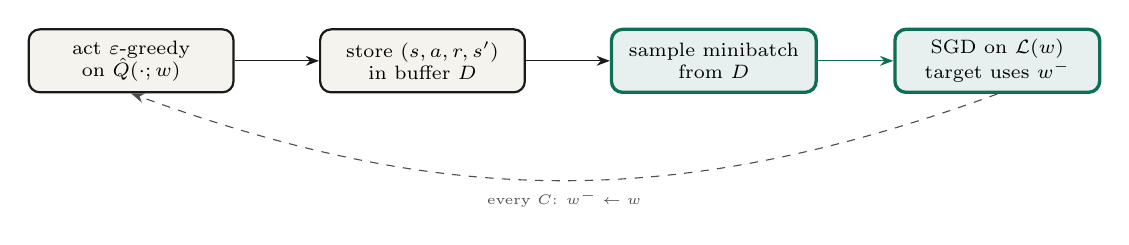
\begin{tikzpicture}[font=\scriptsize, node distance=8pt]
\node[draw=mDarkBrown, thick, fill=mPaleBg, rounded corners, minimum width=2.6cm, minimum height=0.8cm, align=center] (act) at (0,0) {act $\varepsilon$-greedy\\ on $\hat Q(\cdot;w)$};
\node[draw=mDarkBrown, thick, fill=mPaleBg, rounded corners, minimum width=2.6cm, minimum height=0.8cm, align=center] (store) at (3.7,0) {store $(s,a,r,s')$\\ in buffer $D$};
\node[draw=mDarkTeal, very thick, fill=mDarkTeal!10, rounded corners, minimum width=2.6cm, minimum height=0.8cm, align=center] (sample) at (7.4,0) {sample minibatch\\ from $D$};
\node[draw=mDarkTeal, very thick, fill=mDarkTeal!10, rounded corners, minimum width=2.6cm, minimum height=0.8cm, align=center] (update) at (11.0,0) {SGD on $\mathcal{L}(w)$\\ target uses $w^-$};
\draw[-{Stealth}, mDarkBrown] (act) -- (store);
\draw[-{Stealth}, mDarkBrown] (store) -- (sample);
\draw[-{Stealth}, mDarkTeal] (sample) -- (update);
\draw[-{Stealth}, mLightBrown, dashed] (update.south) to[bend left=20] node[below, font=\tiny]{every $C$: $w^- \leftarrow w$} (act.south);
\end{tikzpicture}
\end{center}
\medskip

\pause
Trace the lineage of each box: \emph{act $\varepsilon$-greedy} (Act 2's exploration tax), \emph{$\max$ in the target} (Act 3's off-policy Q-learning), \emph{bootstrap target} (Act 1's TD), \emph{buffer + frozen $w^-$} (Act 4's triad fixes). One loop holds the whole lecture.
\end{frame}

\begin{frame}{What comes after DQN --- one slide of horizon}
The two tricks opened a decade of refinements, each patching a named flaw:
\medskip
\begin{itemize}\setlength\itemsep{2pt}
\item \textbf{Double DQN} --- the $\max$ over-estimates; decouple action-selection from evaluation. \paper{van Hasselt et al., 2016}
\item \textbf{Dueling networks} --- split $\hat Q$ into state-value $+$ advantage; learn ``which states matter'' separately. \paper{Wang et al., 2016}
\item \textbf{Prioritized replay} --- sample high-error transitions more often. \paper{Schaul et al., 2016}
\item \textbf{Rainbow} --- combine them; the sum beats every part. \paper{Hessel et al., 2018}
\end{itemize}
\medskip

\pause
Every one keeps the same skeleton: \emph{sampled Bellman backup} $+$ \emph{$Q$ for model-free greed} $+$ \emph{a stabilizer}. None of them brings back the model --- and none of them works in \alert{continuous action spaces}, where $\max_{a'}$ itself becomes intractable.
\medskip
\begin{center}\large
That wall --- the $\max$ over a continuum --- is exactly where \alert{Lecture 9} begins.
\end{center}
\end{frame}

%==========================================================
\section{Closing}
%==========================================================

\begin{frame}{Where we are --- the cell, filled}
\vspace{2pt}
\begin{center}\footnotesize
\renewcommand{\arraystretch}{1.35}
\begin{tabular}{r|c|c}
 & \textbf{Model-based} & \textbf{Model-free} \\
\hline
\textbf{Static, single} & optimization \;{\scriptsize Lec.\ 1} & bandit \;{\scriptsize Lec.\ 8 intro} \\
\hline
\textbf{Dynamic, discrete, single} & MDP / DP \;{\scriptsize Lec.\ 7 \checkmark} & \cellcolor{mDarkTeal!15}\textbf{value-based RL} \;{\scriptsize Lec.\ 8 \checkmark} \\
\hline
\textbf{Dynamic, continuous, single} & optimal control \;{\scriptsize Lec.\ 9} & policy-based RL \;{\scriptsize Lec.\ 9 $\to$} \\
\end{tabular}
\end{center}
\medskip

\pause
And one repeated move, three times over: \;\textbf{model} $\to$ \textbf{sample}; \;\textbf{wait} $\to$ \textbf{bootstrap}; \;\textbf{table} $\to$ \textbf{function}.
\end{frame}

\begin{frame}{Closing --- the one sentence}
\vfill
\begin{center}\large
Lecture 7 could solve the Bellman equation, because it owned the world.\\[8pt]
Lecture 8 \alert{learned} to solve it ---\\[4pt]
by sampling the expectation, storing $Q$ instead of $V$,\\[4pt]
and replacing the table with a network it could trust.
\end{center}
\vfill
\pause
\footnotesize
From a windy gridworld to human-level Atari with one update rule: the distance between \emph{knowing} the dynamics and \emph{never needing to}. What stays fixed through all of it is the equation Bellman wrote --- we only ever changed what we were allowed to look up.
\end{frame}

\begin{frame}[standout]
Questions?
\end{frame}

%==========================================================
\appendix
%==========================================================

\begin{frame}{Backup 1 --- MC vs.\ TD, the bias--variance ledger}
\footnotesize
Both estimate $V^\pi(s)=\mathbb{E}_\pi[G_t\mid s_t=s]$ from samples; they differ in \emph{what} they sample.
\medskip

\textbf{Monte Carlo target} $G_t = \sum_{k} \gamma^k r_{t+k+1}$.
\begin{itemize}\setlength\itemsep{1pt}
\item \emph{Bias:} none --- $\mathbb{E}[G_t]=V^\pi(s_t)$ exactly.
\item \emph{Variance:} high --- a function of \emph{many} random rewards/transitions along the whole episode.
\end{itemize}
\medskip
\textbf{TD(0) target} $r_{t+1}+\gamma V(s_{t+1})$.
\begin{itemize}\setlength\itemsep{1pt}
\item \emph{Bias:} present --- uses the current (imperfect) estimate $V(s_{t+1})$; unbiased only at the true $V^\pi$.
\item \emph{Variance:} low --- depends on \emph{one} reward and one transition.
\end{itemize}
\medskip
\textbf{The bridge: $n$-step and TD($\lambda$).} Interpolate by bootstrapping after $n$ steps,
$G_t^{(n)} = r_{t+1}+\cdots+\gamma^{n-1}r_{t+n}+\gamma^n V(s_{t+n})$; $n{=}1$ is TD(0), $n{=}\infty$ is MC. TD($\lambda$) averages all $n$ geometrically. The whole family is one dial between \emph{low-bias/high-variance} and \emph{higher-bias/low-variance}.
\end{frame}

\begin{frame}{Backup 2 --- when does tabular Q-learning converge?}
\footnotesize
\textbf{Claim} \paper{Watkins \& Dayan, 1992}: tabular Q-learning converges to $Q^*$ with probability 1, provided
\begin{itemize}\setlength\itemsep{2pt}
\item every state--action pair $(s,a)$ is visited \alert{infinitely often} (the role of exploration, e.g.\ $\varepsilon>0$), and
\item the step sizes satisfy the Robbins--Monro conditions $\sum_t \alpha_t = \infty,\quad \sum_t \alpha_t^2 < \infty$.
\end{itemize}
\medskip
\textbf{Why it holds (sketch).} The Bellman optimality operator
$(\mathcal{T}Q)(s,a) = \mathbb{E}_{s'}[\,r + \gamma\max_{a'}Q(s',a')\,]$
is a $\gamma$-contraction in the sup-norm, so it has a unique fixed point $Q^*$. The Q-learning update is a \alert{stochastic approximation} of $\mathcal{T}$: each step replaces the expectation by one sample. Robbins--Monro step sizes average out the sampling noise; infinite visitation guarantees every entry keeps being corrected. Together they drive $Q \to Q^*$.
\medskip
\textbf{What breaks under approximation.} Replace the table by $\hat Q(\cdot;w)$ and the update is no longer a contraction in any norm the parameters respect --- the projection onto the function class can \emph{expand} distances. That is the formal root of the deadly triad, and the reason DQN needs its two crutches.
\end{frame}

\begin{frame}{Backup 3 --- the function-approximation gradient, in full}
\footnotesize
Linear case $\hat Q(s,a;w) = w^\top \phi(s,a) = \sum_k w_k \phi_k(s,a)$. Per-transition squared TD error:
\[
\text{Err}(w) = \tfrac12\Big(r + \gamma\max_{a'}\hat Q(s',a';w) - \hat Q(s,a;w)\Big)^2.
\]
Differentiate, holding the target fixed (semi-gradient):
\[
\frac{\partial \text{Err}}{\partial w_k}
= -\Big(r + \gamma\max_{a'}\hat Q(s',a';w) - \textstyle\sum_j w_j\phi_j(s,a)\Big)\phi_k(s,a),
\]
\[
\Rightarrow\quad w_k \leftarrow w_k + \alpha\,\Big(r + \gamma\max_{a'}\hat Q(s',a';w) - \hat Q(s,a;w)\Big)\phi_k(s,a).
\]
\medskip
In vector form $w \leftarrow w + \alpha\,\delta\,\phi(s,a)$ --- the tabular update is the special case $\phi(s,a)=\mathbf{e}_{(s,a)}$ (a one-hot indicator), which is why tabular RL is ``just'' function approximation with the most local possible features. For a neural net, $\phi$ becomes $\nabla_w \hat Q(s,a;w)$ and the same line holds.
\end{frame}

\begin{frame}{Backup 4 --- model-based RL, the alternative we set aside}
\footnotesize
The branch we acknowledged in Act~0 and walked away from.
\medskip

\textbf{Estimate the model} from the same stream of experience:
\[
\hat P(s'\mid s,a) = \frac{\#(s,a,s')}{\#(s,a)}, \qquad \hat R(s,a,s') = \text{mean of } r \text{ over } (s,a,\cdot,s').
\]
\textbf{Then solve} the estimated MDP with any Lecture~7 method (value/policy iteration).
\medskip

\textbf{Trade-offs.}
\begin{itemize}\setlength\itemsep{1pt}
\item \emph{Pro --- sample efficiency:} a learned model can be ``replayed'' indefinitely; each real transition informs the value of \emph{many} states through planning.
\item \emph{Con --- model bias:} errors in $\hat P,\hat R$ compound through planning; you optimize for a world that is slightly wrong.
\item \emph{Con --- cost:} estimating a full kernel is far more than estimating the $Q^*$ we actually act on.
\end{itemize}
\medskip
This is why model-free dominated the deep-RL era --- and why Lecture~10 returns to model-based methods only once it can make the learned model carry its weight (planning, Dyna, differentiable control).
\end{frame}

\end{document}
